\section{预测结果、误差与稳健性}\label{sec:prediction_results}

\subsection{总体性能}
基础 ExtraTrees、丰富特征 ExtraTrees 与双分支融合的母体等权 MAE 依次为 0.7469、0.6831 和 0.6668。融合流程在所比较的开发集方案中取得最低观测误差，逐行 MAE 为 0.6510，RMSE 为 0.8842，$R^2$ 为 0.5234。表\ref{tab:v2_main_metrics} 以基础树和丰富特征树为比较起点，同时列出 TabPFN 单分支和两种包含更多候选分支的融合方案，便于评价表示扩展与融合的增量表现。

\begin{table}[htbp]
\centering
\small
\caption{开发集母体分组外层验证结果。每个种子先在合并的五折预测上计算四项指标，再对三个种子取平均。前三项误差使用对数溶解度尺度，$R^2$ 无量纲。}
\label{tab:v2_main_metrics}
\begin{tabular}{lrrrr}
\toprule
模型流程 & 母体等权 MAE & 逐行 MAE & RMSE & $R^2$ \\
\midrule
基础描述符 ExtraTrees & 0.7469 & 0.7491 & 0.9730 & 0.4229 \\
丰富特征 ExtraTrees & 0.6831 & 0.6720 & 0.8981 & 0.5083 \\
TabPFN 单分支 & 0.6827 & 0.6698 & 0.9117 & 0.4933 \\
ExtraTrees 与 TabPFN 融合 & \textbf{0.6668} & \textbf{0.6510} & \textbf{0.8842} & \textbf{0.5234} \\
TabPFN 与双树融合 & 0.6729 & 0.6631 & 0.8882 & 0.5191 \\
五候选分支融合 & 0.6767 & 0.6568 & 0.8899 & 0.5172 \\
\bottomrule
\end{tabular}
\end{table}

\subsection{改进来源与融合增量}
丰富特征树的母体等权 MAE 较基础树降低 0.0638（8.54\%）。以丰富特征树减基础树计算差值，95\% 母体配对区间为 $[-0.1219,-0.0082]$。这项差异对应描述符、模型配置及训练策略共同变化后的整体表现。为进一步区分设计因素，表\ref{tab:v2_tree_pilot} 报告此前三折分组筛查的四个 ExtraTrees 对照。固定 300 棵树、无深度上限、叶节点最小样本数 2、特征采样比例 0.7 以及相同划分后，增加交互特征使 $q=0$ 和 $q=1$ 时的母体等权 MAE 分别下降 0.0127 和 0.0093。逐行等权切换为母体等权训练时，两种表示下的观察降幅分别为 0.0258 和 0.0225。这些比较说明两项设计在该轮筛查中的方向一致。其数值按单一种子和三折划分计算，适合用于理解设计选择。

\begin{table}[htbp]
\centering
\small
\caption{丰富特征 ExtraTrees 的三折开发集筛查。各格为母体等权 MAE，使用同一分组划分、种子 2026 及树参数。}
\label{tab:v2_tree_pilot}
\begin{tabular}{lrr}
\toprule
结构表示 & 逐行等权（$q=0$） & 母体等权（$q=1$） \\
\midrule
丰富描述符拼接 & 0.7112 & 0.6853 \\
拼接、逐元素乘积与绝对差 & 0.6985 & 0.6760 \\
\bottomrule
\end{tabular}
\end{table}

在对齐的外层折外预测中，融合较丰富特征 ExtraTrees 和 TabPFN 的母体等权 MAE 分别减少 0.0163 和 0.0159，相对降幅为 2.39\% 和 2.32\%。对应的 95\% 配对区间分别为 $[-0.0370,0.0001]$ 和 $[-0.0478,0.0178]$（融合减对照）。两个区间都覆盖零，增量收益的稳定性有待锁定方案后的新数据评价。逐条有符号残差的 Pearson 相关系数为 0.909，说明两分支的偏差方向往往相近，融合的价值应结合具体母体的改善与退化判断。

\subsection{母体与目标区间误差}
融合模型的逐母体 MAE 中位数为 0.544，第 90 百分位数为 1.355，最大值为 2.670。与丰富特征树相比，128 个母体中有 61 个误差下降、41 个上升，26 个持平。26 个持平母体位于将 TabPFN 权重设为零的外层折上。与 TabPFN 相比，65 个母体改善，63 个退化。均值变化因此掩盖了母体间差异。

\begin{table}[htbp]
\centering
\small
\caption{融合流程按实测溶解度划分的开发集外层折外误差。记录数和母体数按区间内的唯一观测和母体计数，同一母体可出现在多个区间。各指标在区间内对记录和三个种子等权平均。有符号误差定义为预测值减实测值，正值表示高估。}
\label{tab:v2_target_band_errors}
\begin{tabular}{lrrrr}
\toprule
实测对数溶解度 & 记录数 & 母体数 & MAE & 平均有符号误差 \\
\midrule
$y\leqslant-4$ & 23 & 8 & 2.251 & $+2.250$ \\
$-4<y\leqslant-2$ & 321 & 56 & 0.874 & $+0.784$ \\
$-2<y\leqslant0$ & 824 & 110 & 0.465 & $-0.120$ \\
$y>0$ & 339 & 43 & 0.782 & $-0.772$ \\
\bottomrule
\end{tabular}
\end{table}

误差随实测溶解度区间而变化（表\ref{tab:v2_target_band_errors}）。低值区的 23 条记录平均被高估约 2.25 个对数单位，$y>0$ 的记录则呈低估。以跨种子的平均绝对误差选出误差最大的记录为例，蔗糖在氯仿中、温度原始数值为 25 时，实测对数溶解度为 $-6.234$，三个种子的平均预测为 $-2.536$。对应外层训练部分含 98 条氯仿记录，温度范围为 $[-29.2,55.05]$。即使溶剂和温度落在训练数据覆盖内，目标值极低的未见母体仍可能被明显高估。

\subsection{权重、随机种子与上下文设置}
五个外层折通过内层验证得到的 TabPFN 权重依次为 0.25、0.25、0、0.25、0.50，反映了训练样本变化下的选权差异。在已保存的单分支折外预测上，把 TabPFN 权重固定为 0.25、0.50 或 0.75，得到的母体等权 MAE 分别为 0.6734、0.6708、0.6732（图\ref{fig:v2_prediction_diagnostics}b）。该事后曲线刻画固定权重的敏感程度。主结果 0.6668 对应各折独立地在内层选择权重的验证流程。按种子 17、42、2026 分别汇总，该流程的母体等权 MAE 为 0.6635、0.6679、0.6690，范围宽度为 0.0056；这三个结果来自同一外层划分。

另一项三折筛查固定 TabPFN 的 23 维基础输入及四成员配置，检查训练折内对每个母体设置上下文记录上限的影响。完整上下文的母体等权 MAE 为 0.7252，每个母体最多保留 32 条时为 0.7148，限制至 16 条和 8 条时分别增至 0.7466 和 0.7807。温和裁剪在该筛查中有小幅收益，进一步收紧则伴随误差上升。这些结果描述上下文规模的取舍，正式双分支流程继续使用完整训练折上下文。

\begin{figure}[htbp]
\centering
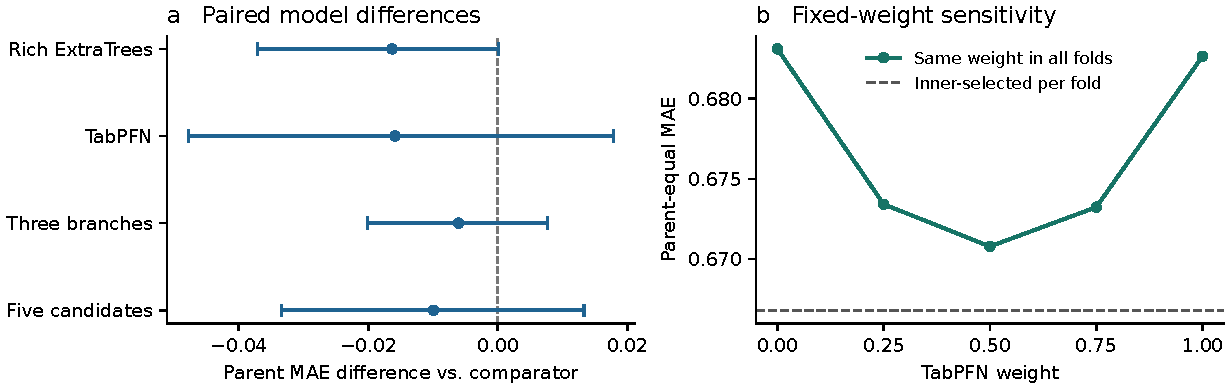
\includegraphics[width=\linewidth]{prediction_diagnostics.pdf}
\caption{融合流程的配对差值及固定权重灵敏度。\textbf{a} 差值为双分支融合减对照的母体等权 MAE，负值表示融合误差较小。区间对 128 个母体配对重采样 10000 次，保存的折外预测保持固定。\textbf{b} 将同一权重用于各外层折的两支折外预测，图中虚线为内层按折选权流程的观测误差。两幅图均基于 1507 条开发记录。}
\label{fig:v2_prediction_diagnostics}
\end{figure}

\subsection{性能与复杂度取舍}
加入 CatBoost 的三候选分支方案和允许五个分支参与选权的方案，母体等权 MAE 分别为 0.6729 与 0.6767。相对这两种方案，双分支的观测差值分别为 $-0.0061$ 和 $-0.0099$，母体配对区间为 $[-0.0201,0.0076]$ 和 $[-0.0334,0.0133]$（图\ref{fig:v2_prediction_diagnostics}a）。五候选方案在各外层折实际启用三个非零分支，表明扩大候选集合也会改变权重选择和配置复杂度。双分支在本次比较中的平均误差较低，部署时需管理的模型也较少，因此被选为应用方案。
